% !TeX spellcheck = fr-FR

\documentclass[10pt,a4paper,notitlepage ]{article}

\usepackage{pfmath}
\usepackage{graphicx}
\usepackage{listings}

\lstset{
	backgroundcolor=\color{yellow!5!white},
	keywordstyle=\color{violet!80!black},
	numbers=left,
	frame=single,
	numberstyle=\tiny\color{violet!80!black},
	escapeinside={\%*}{*)},
	stringstyle=\color{black!20!yellow},
	morecomment=[l][\color{green}]{\$}
}

\title{Systèmes numériques - \textsc{Ernest'O'Clock}}
\date{Premier semestre 2020}
\author{Paul \textsc{Fournier}, Juliette \textsc{Schabanel}, Samuel \textsc{Vivien}}


\begin{document}
	\selectlanguage{french}
	\pagenumbering{gobble}
	\maketitle
	\pagebreak
	\pagenumbering{roman}
	\tableofcontents
	\pagebreak
	\pagenumbering{arabic}
	
	\section{Compilation $\tt{.net} \rightarrow \tt{.c}$}
	
	\subsection{Motivations}
	
	De prime abord, nous avions implémenté un simulateur de netlist, codé en \texttt{OCaml}, mais nous avons décidé de changer et de produire un code \texttt{C} ayant le même comportement que la netlist d'entrée, et ce pour deux raisons.
	\begin{enumerate}
		\item Les performances de \texttt{C}, en particulier grâce à l'optimisation apportée par \texttt{gcc}.
		\item Le côté bas niveau permet de gérer plus facilement les entrées/sorties de l'ordinateur/simulateur/émulateur.
		\item Avons-nous mentionné \texttt{gcc} ?
	\end{enumerate}
	
	\subsection{Implémentation}
	
	Le compilateur est implémenté en \texttt{OCaml}, parce que la plupart du code en amont l'était déjà, ce qui permet d'éviter des interfaces inutiles et lourdes.
	
	L'idée est assez simple finalement, en \texttt{C}, on alloue un énorme tableau, dont chaque case est un fil, un tableau par RAM, et un tableau par ROM. Les opérations sur les netlist se transforment alors par un isomorphisme presque immédiat en opération sur les tableaux.
	
	\subsubsection{Les fils}
	
	Nous donnons ici rapidement les idées derrière la traduction des opérations sur des fils simples.
	
	\begin{center}
		
	\begin{tabular}{|c|c|}
		\hline
		Opérations sur les fils & Opérations sur les tableaux \\
		\hline
		Constante (\texttt{true} ou \texttt{false})& Constante ($0$ ou $1$)  \\
		\hline
		\texttt{not ?}& \texttt{!?}  (nb: plus rapide qu'un \texttt{xor})\\
		\hline
		\texttt{and} & \texttt{\&}  \\
		\hline
		\texttt{or}& \texttt{|} \\
		\hline
		\texttt{xor}& \texttt{\^} \\
		\hline
		\texttt{a nand b }& \texttt{!(a \& b)} \\
		\hline
		\texttt{mux s b a}& \texttt{s?a:b} \\
		\hline
		\texttt{reg}&Assignation\\
		\hline
	\end{tabular}
	
	\end{center}

	\subsubsection{Les RAM}
	
	Chaque RAM est un tableau. La lecture est simplement la lecture des cases du tableau, et l'écriture, sans grande surprise, l'écriture dans les cases du tableau.
	
	Les opérations sont effectuées bit à bit, il pourrait donc y avoir quelques optimisations à effectuer de ce côté là (en écrivant par blocs de puissances de deux par exemple).
	
	Si une adresse non valide est spécifiée, le CPU lève un \texttt{SEGFAULT}.
	
	\subsubsection{Les ROM}
	
	Étant immuables, les ROM sont définies en dur dans le code \texttt{C} généré par le compilateur (par exemple, aux alentours des lignes ~150 du code produit pour notre CPU, on peut trouver la ROM comprenant le code à exécuter, telle les disquettes des anciens).
	
	On peut donc y lire, comme dans une RAM, et planter sur un \texttt{SEGFAULT} si on fait n'importe quoi.
	
	
	\section{Interface homme machine}
	
	Nous allons ici détailler la façon dont nous avons implémenté l'interface entre le microprocesseur, qui, après calcul, donne une représentation du temps sous format sept segments.
	
	\begin{figure}[h]
		\centering
		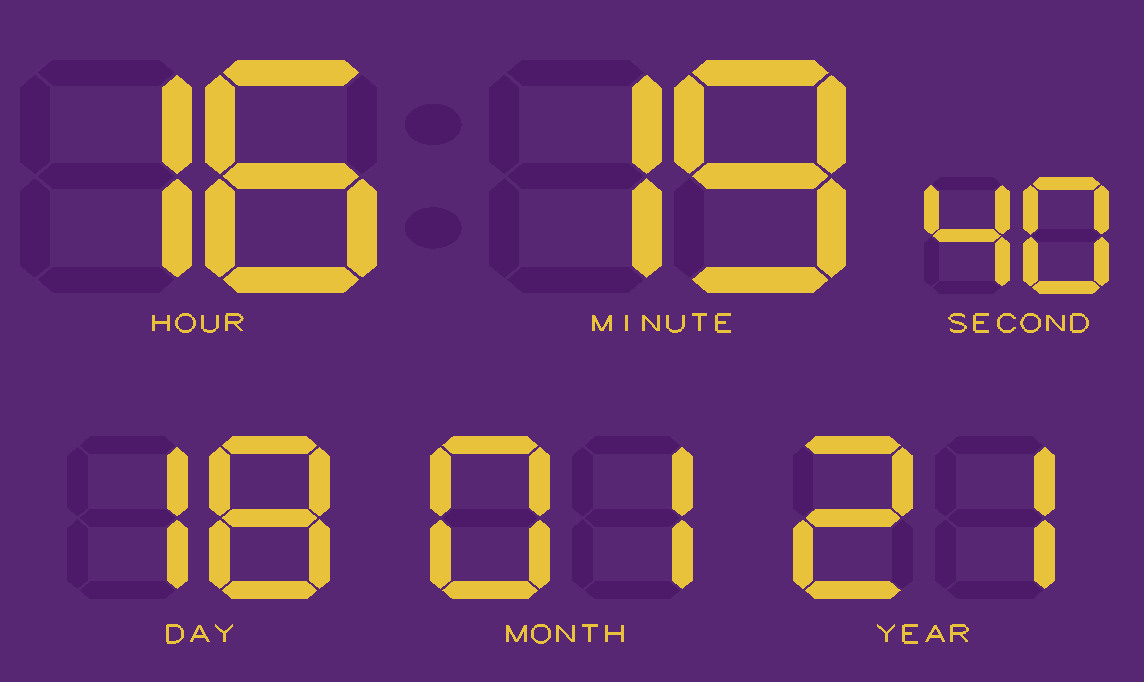
\includegraphics[width=0.7\linewidth]{2021-01-18_16-19}
		\caption{Capture d'écran de la sortie de l'horloge}
		\label{fig:2021-01-1816-19}
	\end{figure}
	
	Commençons par expliquer comment nous avons réalisé l'affichage en lui-même.
	
	\subsection{Programmation graphique de l'horloge}
	
	Ils a donc d'abord fallu décider d'une façon d'encoder en mémoire les segments. Pour cela, chaque chiffre est représenté par un mot de $7$ bits (donc en pratique par un octet). La figure ci-dessous détaille quel bit correspond à quel segment (avec le mot indicé comme $b_0b_1b_2b_3b_4b_5b_6b_7$).
	
	\begin{figure}[h]
		\centering
		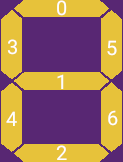
\includegraphics[width=0.3\linewidth]{segments}
		\caption{Encodage des segments}
		\label{fig:segments}
	\end{figure}
	
	L'interface s'est effectuée directement par une lecture dans la RAM. Une section "MMIO" a été définie et réservée pour cela. C'est concrètement du repiquage de fil de la mémoire vers un afficheur à cristaux liquide, mais virtualisé dans le code \texttt{C}.
	
	Maintenant qu'on a récupéré le statut "on/off" de chaque segment, il est temps de l'afficher !
	
	Nous avons choisi d'utiliser \texttt{OpenGL} comme libraire graphique. Ce choix a été motivé principalement parce que nous avions déjà (un peu) d'expérience avec cette librairie et que cela permettait de gagner en efficacité pendant la production. Par ailleurs, c'est une libraire répandue et connue, ce qui nous a évité de chercher pendant des heures comment faire pour afficher quelques bâtons sur un écran. Cependant, bien que nous avons voulu, en gardant le code assez simple, optimiser autant que faire se peut la vitesse d'affichage, $\tt{OpenGL}$ restant une libraire de rendu 3D à l'origine, il est évident que les opérations matricielles à répétition qu'engendrent le positionnement des différents éléments sur l'écran sont probablement sous-optimaux par rapport à une librairie spécialisée dans l'affichage rapide de forme géométrique simples en deux dimensions.
	
	Comme il y a 3 formes à afficher (segment horizontal, segment vertical et point), nous avons décidé d'utiliser les "display list" pour stocker en mémoire les formes et les répliquer plus rapidement par la suite. Nous n'avons pas relevé expérimentalement de différence, mais c'est considéré comme une bonne pratique par l'ouvrage qui nous a servi de référence (OpenGL programming guide - The official guide to learning OpenGL). Ensuite, c'est juste du placement minutieux de chaque segment. Les détails précis de la position ne seront pas explicités ici (long, moche, pénible, et inutile au propos), ils sont cela dit consultable depuis le code source, pour nos lecteurs masochistes. En fait, en interne, à chaque placement, \texttt{OpenGL} fait un produit matriciel $4\times 4$, ce qui pourrait en pratique être simplifié en utilisant autre chose qu'un moteur 3D.
	
	Finalement, à chaque frame, \texttt{OpenGL} affiche $7\times 12$ segments, et deux points, de la couleur adaptée (allumé, éteint, selon le seul code couleur qui vaille la peine d'être implémenté) en plus du texte.
	
	\subsection{Entrées du microprocesseur}
	
	Afin d'interagir avec le monde, le microprocesseur doit aussi prendre des entrées. Pour le projet d'horloge, il s'agit d'une information d'initialisation - l'heure initiale -, et d' une information en temps réel - la parité de la seconde actuelle.
	
	L'heure initiale est donnée sous la forme d'un entier 32 bits, encodé classiquement, contenant le nombre de secondes depuis le premier Janvier 1970 (UNIX epoch). Le microprocesseur fait toutes les conversions nécessaires en interne.
	
	Ensuite, le bit de parité de la seconde en cours (qui sert aussi pour faire clignoter les deux points séparant les minutes des secondes), est calé entre deux paquets de sept bits dans le MMIO, bien au chaud.
	
	\subsection{Optimisations pour le mode \textit{hyper-vitesse}}
	
	Lors des premiers tests, nous avons remarqué que l'affichage était le facteur limitant en termes de vitesse d'affichage, pas le CPU. C'est pour cela que nous avons voulu passer un peu de temps à réduire le temps passé à afficher des choses à l'écran.
	
	Pour cela, nous avons ajouté un bit dans l'interface MMIO (toujours calé entre deux blocs de sept), qui est envoyé par le CPU lorsque les calculs sont terminés pour une unité de temps, qui dit concrètement au front-end "fin de la pause, il faut mettre à jour l'affichage de l'heure". Une fois que l'affichage est réalisé, ce bit est remis à zéro.
	
	\subsection{Lecture des inputs de l'utilisateur}
	
	Les entrées clavier de l'utilisateur sont lues lors de l'exécution de l'horloge et que le processus est en avant-plan. Actuellement, tout ce qui est vérifié est l'appui des touches \texttt{Q} et \texttt{MAJ} en simultané, ce qui ferme le programme.
	
	\subsection{Autres idées non implémentées}
	
	Nous avions d'autres projets pour cette partie d'interface. En particulier, nous voulions enrichir l'entrée utilisateur. Des tests en local (\texttt{hexdump}, entre autres) nous ont permis de conclure qu'il était, effectivement, possible de faire ce qui est ni plus ni moins qu'un keylogger en lisant directement dans \texttt{/dev/input}. Nous avons testé, et il était possible de récupérer les informations de :
	\begin{itemize}
		\item Trackpad
		\item Clics
		\item Clavier
		\item Manette de \textsc{Nintendo} Switch\texttrademark\ type Game Cube (connectique USB)
	\end{itemize}
	
	Le code utilisé pour tester peut être trouvé en annexe.
	Il aurait alors été possible, avec un peu de traitement, certes, de donner des informations plus complexes au CPU. 
	
	Nous aurions aussi voulu modifier le système d'affichage pour pouvoir avoir du contrôle directement sur les pixels mêmes de l'écran. Là aussi, nous aurions voulu aller fouiner du côté du noyau Linux, mais c'est une magie encore trop ésotérique pour nous. Nous aurions aussi pu chercher une librairie qui gère de l'affichage 2D, mais le temps nous a manqué.
	
	L'objectif final aurait été de pouvoir avoir une machine qui a des performances comparables à celles des premières consoles de jeu, et montrer ses performances en implémentant un petit jeu type Snake ou Pong.
	
	De manière orthogonale, nous aurions aussi aimé, quitte à utiliser \texttt{OpenGL}, pouvoir faire profiter l'utilisateur de l'horloge d'un environnement 3D composé essentiellement d'une table de chevet sur laquelle repose un radio-réveil (notre horloge).
	
	
	\begin{figure}
	\begin{lstlisting}[language=C, frame=single, caption={Keylogger test}]
#include <stdlib.h>
#include <stdio.h>
#include <string.h>
#include <errno.h>
#include <linux/input.h>
#include <sys/types.h>
#include <sys/stat.h>
#include <fcntl.h>
#include <libevdev/libevdev.h>
#include <libevdev/libevdev-uinput.h>

int main(){
	
	struct libevdev *dev = NULL;
	int fd;
	int rc = 1;
	
	// keyboard : /dev/input/event3
	//fd : file descriptor
	fd = open("/dev/input/event3", O_RDONLY|O_NONBLOCK);
	// rc : return code
	// modifies *dev such that it is hooked to the /dev/input file
	rc = libevdev_new_from_fd(fd, &dev);
	if (rc < 0) {
		//error happenned
		fprintf(stderr, "Failed to init libevdev (%s)\n", strerror(-rc));
		exit(1);
	}
	printf("Input device name: \"%s\"\n", libevdev_get_name(dev));
	printf("Input device ID: bus %#x vendor %#x product %#x\n",
	libevdev_get_id_bustype(dev),
	libevdev_get_id_vendor(dev),
	libevdev_get_id_product(dev));
	
	do {
		struct input_event ev;
		rc = libevdev_next_event(dev, LIBEVDEV_READ_FLAG_NORMAL, &ev);
		if (rc == 0)
		printf("Event: %s %s %d\n",
		libevdev_event_type_get_name(ev.type),
		libevdev_event_code_get_name(ev.type, ev.code),
		ev.value);
	} while (rc == 1 || rc == 0 || rc == -EAGAIN);
	0;
}
	\end{lstlisting}
	\end{figure}
\end{document}